\section{Ziel des Versuches}
Ziel des Versuches ist es die Funktionsweise eines He-Ne-Lasers zu verstehen und den Umgang mit diesem zu üben. Dafür soll die Wellenlänge des Lasers und die maximale Resonatorlänge gefunden werden. Außerdem soll die Intensität von zwei TEM-Moden und der Polarisation ausgemessen werden.


\section{Theoretische Grundlage}
\subsection{Aufbau eines Gaslasers}
Im folgenden wird kurz der Aufbau und die Funktionsweise eines Lasers (\textbf{L}ight \textbf{A}mplification by \textbf{S}timulated \textbf{E}mission of \textbf{R}adiation) erklärt, mit besonderem Augenmerk auf die Gaslaser (He-Ne-Laser). \\
Das \textbf{aktive Lasermedium} des Lasers bestimmt das Strahlungsspektrum. Dafür muss das Lasermedium so manipuliert werden, dass das Strahlungsfeld der einfallenden Strahlung mit dem Gasgemisch wechselwirkt und die Strahlung verstärkt wird. Damit das passiert muss mehr induzierte Emission auftreten als spontane Emission. \\
Nach der Boltzmann-Verteilung ist der Grundzustand, in einem Gas, im thermischen Gleichgewicht stärker besetzt als die angeregten Zustände. Also ist die Besetzungszahl $n_1$ für den Grundzustand größer als die Besetzungszahl $n_2$ für den ersten angeregten Zustand. Vereinfachend kann ein zwei Niveau-System angenommen werden, dann können die Ratengleichungen für die Besetzungszahlen wie folgt formuliert werden:

\begin{align}
	\frac{d\,n_1}{d\,t} = - &\underbrace{n_1\,B_{12}\,\rho}_{\dot{N}_\text{A}} + \underbrace{n_2\,B_{21}\,\rho}_{\dot{N}_\text{IE}} + \underbrace{n_2\,A_{21}}_{\dot{N}_\text{E}}\ \ \text{und}\\
	\frac{d\,n_2}{d\,t} = \ \ \ &\overbrace{n_1\,B_{12}\,\rho}_{} - \overbrace{n_2\,B_{21}\,\rho}_{} - \overbrace{n_2\,A_{21}}_{}
\end{align}

Wobei $\dot{N}_\text{A}$ der Niveauübergang für die Absorbtion, $\dot{N}_\text{IE}$ für die induzierte Emission und $\dot{N}_\text{E}$ für die spontane Emission (siehe Abbildung \eqref{fig:Emission}) ist. Die Einsteinkoeffizienten $A_{21}$, $B_{12}$ und $B_{21}$ sind Konstanten und geben die Übergangswahrscheinlichkeit von dem Grundzustand in den ersten angeregten Zustand an und $\rho$ ist die Energiedichte des Strahlungsfeldes. Damit mehr induzierte Emission auftritt als die spontane Emission muss eine Besetzungsinversion erschaffen werden. Es müssen also mehr Atome im höher energetischen Zustand sein als im Grundzustand. Dies wird über eine permanente Zufuhr von elektrischer Energie in das Lasermedium erzeugt. \\
Dieser Vorgang wird als \textbf{Pumpen} bezeichnet. Bei einem He-Ne-Laser werden zunächst die Helium-Atome mittels elektrischer Entladung angeregt. Dann Stoßen die angeregten Helium-Atome mit den Neon-Atomen, wodurch Energie auf die Neon-Atome übertragen wird und diese danach überwiegend das 3s-Orbital besetzen. Bei dem Übergang von dem 3s-Orbital in das 2p-Orbital (Grundzustand) wird ein Photon mit der charakteristischen Wellenlänge $\lambda = 632,8$nm emittiert.

\begin{figure}[H]
	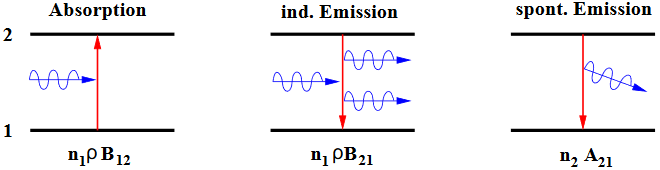
\includegraphics[width=\linewidth]{Bilder/Emission.PNG}
	\caption{Schematische Darstellung der drei möglichen Niveauübergänge. \cite{V61}}
	\label{fig:Emission}
\end{figure}

Diese Photonen regen nun die induzierte Emission an, damit dieser Vorgang so oft wie möglich stattfindet wird der \textbf{Resonator} verwendet. Der Resonator besteht aus zwei gegenüberstehenden Spiegeln und in der Mitte ist das Lasermedium in einer Laserröhre (siehe Abbildung \eqref{fig:Laser}). Der Resonator sorgt dafür, dass das Licht so oft wie möglich durch das Lasermedium läuft und dadurch verstärkt wird (die Verstärkung wächst exponentiell mit der Lauflänge im Lasermedium). Die Stabilität des Resonators ist über die Spiegelparameter $g_\text{i}$ definiert und folgt der Bedingung:
\begin{align}
	0 \le g_1 \cdot g_2 \le 1 \ .
	\label{eqn:Stab}
\end{align}
Die Spiegelparameter sind über
\begin{align}
	g_\text{i} = 1 - \frac{L}{r_\text{i}}
\end{align}
gegeben, wobei $L$ der Abstand zwischen den Spiegeln ist und $r_\text{i}$ der Spiegelradius ist.

\begin{figure}[H]
	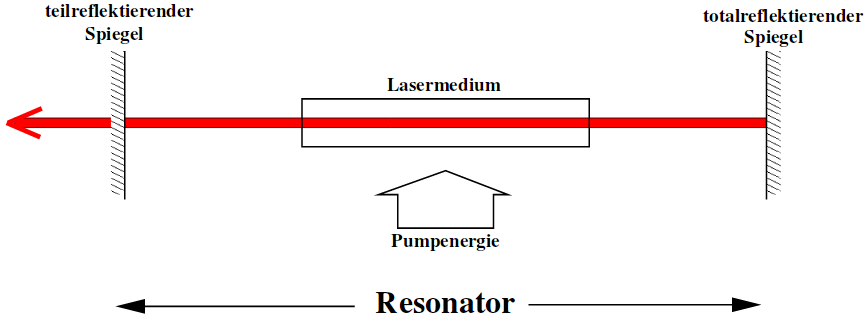
\includegraphics[width=\linewidth]{Bilder/Resonator.png}
	\caption{Schematische Darstellung eines offenen Lasers. \cite{V61}}
	\label{fig:Laser}
\end{figure}

Da $L >> \lambda$ gilt, erfüllen viele Frequenzen die Resonanzbedingung einer stehenden Welle in dem Resonator. Das heißt es bilden sich longitudinale Wellen mit der Knotenzahl $q$ aus. Desweiteren kommen transversale Schwingungen hinzu, mit den Knotenzahlen $p$ und $l$, welche durch Unebenheiten, Verkippungen und kleinen Fehlern in den Spiegeln entstehen. Die skalare Feldverteilung wird durch die transversalen Schwingungen dominiert. \\
Die Eigenschwingungen des Resonators werden als TEM$_{lqp}$-Moden bezeichnet. TEM steht dabei für transversale elektromagnetische Mode. Demnach ist die TEM$_{00}$ die Mode mit der höchsten Symmetrie und den niedrigsten Verlusten.

\subsection{Eigenschaften eines Lasers}
Licht wird als Laser bezeichnet wenn es drei wichtige Eigenschaften hat. Es muss monochromatisch sein und eine hohe Intensität und Kohärenz haben. Desweiteren spielt die Polarisation des Lasers eine Rolle. Auf diese Eigenschaft des Lasers wird im folgenden genauer eingegangen. \\
\textbf{Kohärenz} liegt vor wenn die Phasenverschiebung der Wellenzüge an einem festen Ort zeitlich konstant ist oder wenn sich die Phase gesetzmäßig mit der Zeit ändert.
Das bedeutet, dass die Kohärenz ein Maß für die Interferenzfähigkeit zweier Wellen ist. \\
Die \textbf{Intensität} $I_\text{lpq}$ beschreibt die Leistung pro Fläche welche von dem Laser ausgestrahlt wird und ist proportional zu dem Betragsquadrat der Feldverteilung $E_\text{lpq}$.
\begin{align*}
	I_\text{lpq} \propto |E_\text{lpq}|^2 \ .
\end{align*}
Die Indizes $l$, $p$ und $q$ geben die Anzahl der Knotenpunkte an, welche sich in dem Resonator ausbilden. Um genaueres über die Intensität sagen zu können muss zunächst die Feldverteilung näher betrachtet werden. Für einen konfokalen Resonator mit runden Spiegeln ist die Feldverteilung durch

\begin{align*}
	E_\text{lpq} \propto &\frac{\cos(l\varphi)\,(2\rho)^2}{(1+Z^2)^\frac{1+l}{2}}\, L_p^q\left(\frac{(2\rho)^2}{1+Z^2}\right)\,\exp \left(-\frac{\rho^2}{1+Z^2} \right) \\
	&\exp \left(-i\left(\frac{R\pi(1+Z)}{\lambda}+ \frac{\rho^2Z}{1+Z^2}- (l+2p+1)\left(\frac{\pi}{2}-\arctan \left(\frac{1-Z}{1+Z} \right) \right)\right)\right) \\
	&\text{mit:}\ \ \rho = \left(\frac{2\pi}{R\lambda} \right)^\frac{1}{2} \ \ \text{und} \ \ Z = \frac{2z}{R}
\end{align*}

gegeben. Darin steht $L_p^q(u)$ für das Laguerre-Polynom. \\
Allerdings lässt sich die Intensität der TEM$_{00}$ Grundmode zu
\begin{align}
	I(r) = I_0\,\exp \left(\frac{-2\,r^2}{w^2} \right)
\end{align}
vereinfachen. \\
Die \textbf{Polarisation} tritt nur bei Transversallwellen auf und beschreibt die Richtung der Schwingung. Dabei steht der Wellenvektor senkrecht auf der Ausbreitungsrichtung. Wenn sich der Wellenvektor nur in Ausbreitungsrichtung verschiebt, spricht man von einer linearen Polarisation. Von zirkularer Polarisation spricht man wenn sich der Wellenvektor mit gleich bleibender Geschwindigkeit und konstantem Betrag um eine Achse dreht. In einem Laser wird die Polarisation durch optische Bauteile erreicht, zum Beispiel Brewster-Fenster. \\
Für die \textbf{Beugung von Laserstrahlen} gilt unter der Annahme, dass der Abstand $L$ zwischen dem Beugungsgitter und dem Schirm viel Größer ist als der Abstand $a$ zwischen den Beugungsmaxima ($L >> a$), die Fraunhofer Näherung. Mit Hilfe der Abbildung \eqref{fig:BeugungAmSpalt} kann die Wellenlänge $\lambda$ zu
\begin{align}
	\lambda = s\cdot\sin\varphi
	\label{eqn:lambda}
\end{align}
bestimmt werden, wobei $s = \frac{1}{g}$ der Gitterkonstanten enspricht und $\varphi$ der Beugungswinkel ist. Wenn jetzt noch die Einschränkung getroffen wird, dass nur kleine Beugungswinkel betrachtet werden kann
\begin{align}
	\sin\varphi \approx \tan\varphi = \frac{a}{L}
\end{align}
genähert werden. Damit kann die Wellenlänge eines Lasers über
\begin{align}
	\lambda \approx \frac{a}{L\,g}
	\label{eqn:lambda}
\end{align}
bestimmt werden.

\begin{figure}[H]
	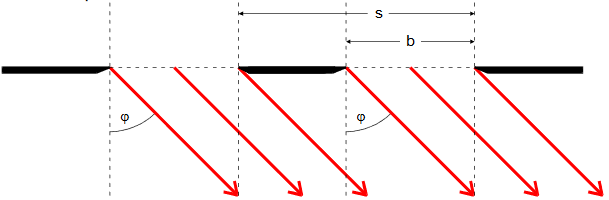
\includegraphics[width=\linewidth]{Bilder/BeugungAmSpalt.PNG}
	\caption{Schematische Darstellung der Fraunhofer Näherung am Mehrfachspalt. \cite{V406}}
	\label{fig:BeugungAmSpalt}
\end{figure}


\subsection{Fehlerrechnung}
Sämtliche Fehlerrechnungen werden mit Hilfe von Python 3.4.3 durchgeführt.
\subsubsection{Mittelwert}
Der Mittelwert einer Messreihe $x_\text{1}, ... ,x_\text{n}$ lässt sich durch die Formel
\begin{equation}
	\overline{x} = \frac{1}{N} \sum_{\text{k}=1}^\text{N} x_k
	\label{eqn:ave}
\end{equation}
berechnen. Die Standardabweichung des Mittelwertes beträgt
\begin{equation}
	\Delta \overline{x} = \sqrt{ \frac{1}{N(N-1)} \sum_{\text{k}=1}^\text{N} (x_\text{k} - \overline{x})^2}
	\label{eqn:std}
\end{equation}

\subsubsection{Gauß'sche Fehlerfortpflanzung}
Wenn $x_\text{1}, ..., x_\text{n}$ fehlerbehaftete Messgrößen im weiteren Verlauf benutzt werden, wird der neue Fehler $\Delta f$ mit Hilfe der Gaußschen Fehlerfortpflanzung angegeben.
\begin{equation}
	\Delta f = \sqrt{\sum_{\text{k}=1}^\text{N} \left( \frac{ \partial f}{\partial x_\text{k}} \right) ^2 \cdot (\Delta x_\text{k})^2}
	\label{eqn:var}
\end{equation}

\subsubsection{Lineare Regression}
Die Steigung und y-Achsenabschnitt einer Ausgleichsgeraden werden gegebenfalls mittels Linearen Regression berechnet.
\begin{equation}
	y = m \cdot x + b
	\label{eqn:reg}
\end{equation}
\begin{equation}
	m = \frac{ \overline{xy} - \overline{x} \overline{y} } {\overline{x^2} - \overline{x}^2}
	\label{eqn:reg_m}
\end{equation}
\begin{equation}
	b = \frac{ \overline{x^2}\overline{y} - \overline{x} \, \overline{xy}} { \overline{x^2} - \overline{x}^2}
	\label{eqn:reg_b}
\end{equation}
